\scanpage{50}
\margin{10.12.1965}

Cher Deligne,

\figure{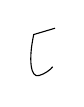
\begin{tikzpicture}[x=0.1cm,y=0.1cm]\draw (3,6)--(0.3,5.2)..controls(-0.4,2)and(-0.1,-0.4)..(1,0)..controls(1.7,0.2)and(2.4,0.7)..(2.7,1.1);\end{tikzpicture}}
Je vous propose une simplification pour la démonstration du théorème de dualité, qui permet d'éviter tout recours au théorème de pureté relative. Vous vous rappelez qu'on était réduit au cas où $f:X\quad Y$ est de dimension relative 1, $F=A_X$ et $G=A_Y$. Le procédé de passage à la limite de Exp VI, par.6, permet de supposer la base noethérienne, et même si on y tien de dimension finie (car de type fini sur $\underline Z$). On raisonne par récurrence sur $n=\dim X$. Si $n=0$, on sait le vérifier. Supposons le théorème démontré en dimension $<n$. Se localisant sur Y, on peut supposer Y strictement local. Alors, si y est son point fermé, on a $\dim(Y-y)\quad n$, et comme on est réduit à prouver le théorème séparément pour $X\times_Y(Y-y)$ et $X\times_Y y$, on gagne. - Autre remarque: le théorème de dualité peut se démontrer, essentiellement de la même façon et avec le même énoncé, pour un morphisme lisse $f:X\quad Y$ compactifiable, lorsque Y est muni d'un faisceau d'anneaux A quelconque tel que il existe un entier n premier aux caractéristiques \unsure{résidueales|résiduelles} annulant A, et X d'un faisceau d'\unsure{anneaux|anneaus} B, et f étant donné comme morphisme de (X,B) dans (Y,A), de sorte qu'on a un \inserted{homo}morphisme de faisceau d'anneaux $f^{-1}(A)\quad B$. On définit alors
\[
f^{!}(K^{\bullet})=R\,\underline{\operatorname{Hom}}^{\bullet}_{f^{-1}(A)}(B,f^{-1}(K)\otimes T_{X/Y}\quad 2d).
\]
La définition de l'homomorphisme trace et la démonstration du théorème de dualité se décomposent alors en le cas où $f^{-1}(A)\quad B$ est un isomorphisme, qui se traite comme le cas $A=(\underline Z/n\underline Z)_Y$, et le cas où $f=\operatorname{id}$, qui est trivial. Je pense qu'il vaut le coup d'inclure cette forme générale du théorème de dualité, soit de prime abord, soit à la fin dans un numéro-ratrappage. Je n'ai pas regardé si par hasard il pourrait se déduire du cas particulier
\margin{49}
